% ----------------------------------------------------
% Literature Review
% ----------------------------------------------------

\chapter{Literature Review}\label{ch:literature}

\section{A Brief History of Salinity}\label{sec:a-brief-history-of-salinity}
The most commonly understood definition of salinity relates it to the total amount of dissolved \textit{salts} in a solution, however, salinity's definition has had several more complex iterations over the years.
One of the first definitions of salinity was the total amount of dissolved \textit{material} in grams in one kilogram of water~\cite{stewart_introduction_to_physical_oceanography_2004}.
This is a dimensionless quantity that was expressed in \gls{ppt} or $g.kg^{-1}$ where most ocean's salinity fell between 34.60\gls{ppt} and 34.80\gls{ppt} as shown in \reffig{fig:ocean_salinity_temperature_quantity}.
\begin{figure}[h]
    \centering
    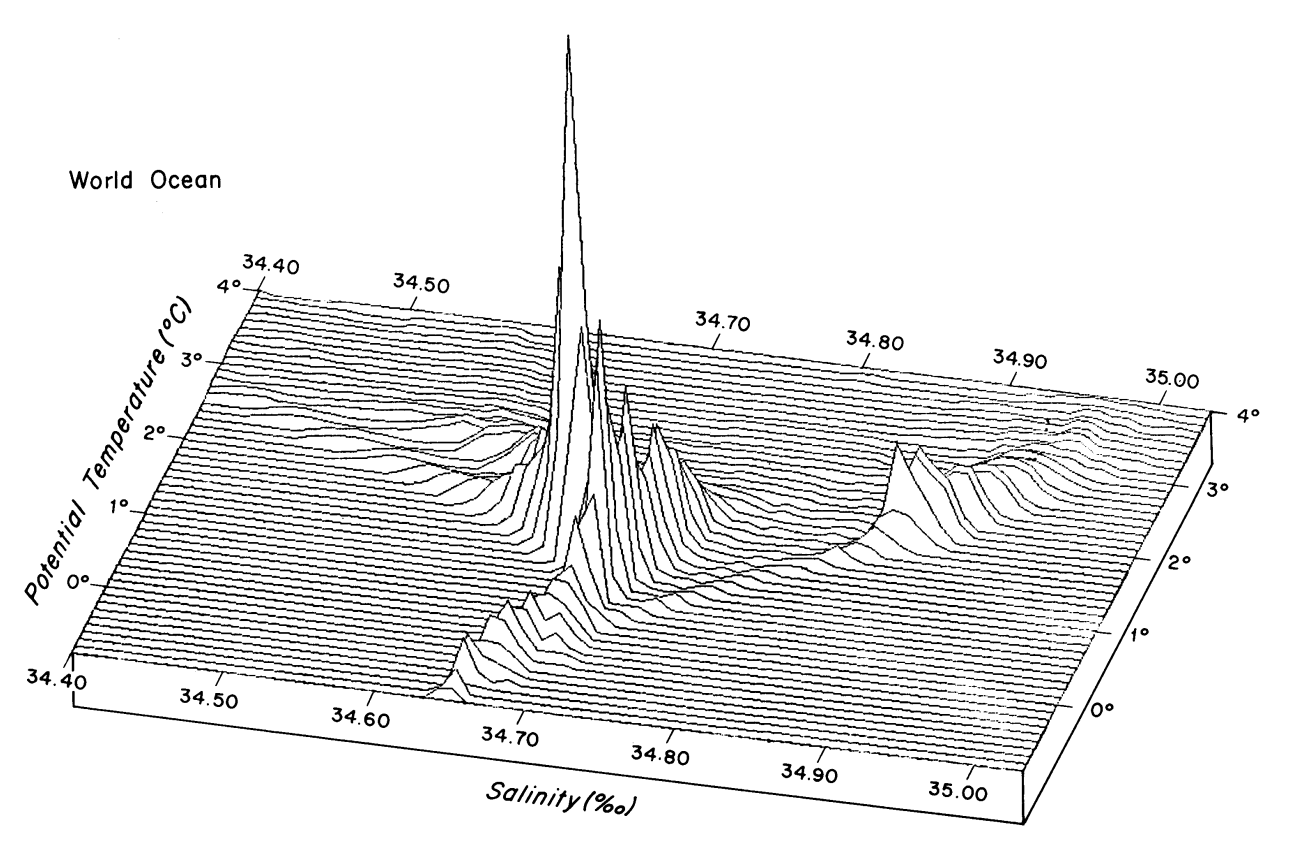
\includegraphics[width=0.75\textwidth]{Figures/ocean_salinity_temperature_quantity}
    \caption{Histogram showing the volume of ocean water relative to temperature and salinity bins. The highest peak corresponds to a volume of 26 million cubic kilometres of ocean water~\cite{worthington_ocean_graphs_1981}.}
    \label{fig:ocean_salinity_temperature_quantity} %chktex 24
\end{figure}\newline
The problem with this definition of salinity lay with its testability.
Trying to obtain the mass of the dissolved material through evaporation removed certain compounds making this method inaccurate~\cite{sverdrup_ocean_physics_and_chemistry_1942} and other methods of isolating the mass of the dissolved material had similar issues. 
Salinity needed to be redefined in a way that was easily and reliably testable which led to the next definition of salinity which related salinity related it to the amount of chlorine present in the water, or the chlorinity of the water and in 1969, salinity was redefined to be directly proportional to the chlorinity of the water~\cite{stewart_introduction_to_physical_oceanography_2004}.
The calculation of salinity from chlorinity is further discussed in~\refsec{subsec:salinity-from-chlorinity}.

Around the same time as the salinity-chlorinity relationship was established, oceanographers had begun experimenting with using conductivity to measure salinity.
Conductivity was found to be more precise and significantly easier to measure than the titration required to measure chlorinity~\cite{lewis_salinity_definition_and_calculation_1978}.
In 1978, the Practical Salinity Scale was established and salinity was redefined to be related to conductivity which is the current definition of salinity\cite{lewis_salinity_definition_and_calculation_1978}.
This relationship also included terms for temperature and depth as these affect the conductivity of an electrolyte solution~\cite{zheng_electrical_conductivity_of_ocean_2017}.

The Practical Salinity Scale uses its own dimensionless units of salinity which are not interchangeable with \gls{ppt} in the current definition of salinity.
Although the Practical Salinity Scale is sometimes given in \gls{psu}, it is more technically correct to refer to it as a certain Practical Salinity `on the Practical Salinity Scale PSS-78'~\cite{lewis_salinity_definition_and_calculation_1978}.
The calculation of salinity from conductivity is further discussed in~\refsec{sec:salinity-conductivity-relationship}.

% \section{The Uses of Salinity Measurements}\label{sec:the-uses-of-salinity-measurements}
% oceanography, speciation, conservation, habitation, water quality (drinking, agriculture, industrial), aquaculture, desalination.
% antarctic ice.

\section{Salinity Measurement Methods}\label{sec:salinity-measurement-techniques}

Salinity has had a long history of being measured using a variety of methods with varying degrees of accuracy.
Currently, the most common method of measuring salinity is through the use of a \gls{ctd} instrument, but there are several other methods to achieve this, most of which have been developed over the last 3 decades.

\subsection{Salinity from Chlorinity}\label{subsec:salinity-from-chlorinity}

The chemical composition of ocean water with a salinity of 35\gls{ppt} contains 19.35\gls{ppt} of Chlorine and 10.77\gls{ppt} of Sodium with the next most common ions only accounting for just above 3\gls{ppt} of the total dissolved solids in the water~\cite{britannica_seawater_encyclopaedia_2024}.
This allowed oceanographers to estimate that the salinity of ocean water was directly proportional to the amount of chlorine in the water.
The chlorinity of a solution had an established definition which was `the mass of silver required to precipitate completely the halogens in $0.328\ 523\ 4 kg$ of the ocean-water sample'~\cite{wooster_redefinition_of_salinity_1969} which could be tested using titration.
In 1969, an accurate relationship between these was established by~\refref{wooster_redefinition_of_salinity_1969} and thus salinity $S$ was redefined using chlorinity $Cl$ as shown in~\refeqn{eqn:salinity-chlorinity}.
\begin{equation}\label{eqn:salinity-chlorinity}
    S (\text{\gls{ppt}}) = 1.80655 \times~Cl (\text{\gls{ppt}})
\end{equation}
\textit{accuracy achieved?, device?, limitations?}

\subsection{Salinity from Conductivity}\label{subsec:salinity-from-conductivity}

The conductivity of a liquid is a measure of the ability of the water to conduct an electrical current which is related to the number of free electrons present in the liquid which is in turn related to the number of ions present in the liquid.
In the case of salt water, the ions present are from the dissolved material which is what salinity was previously defined on.
The relationship between salinity and conductivity takes into account all the ions present in the water and thus was a more apt measure of salinity than chlorinity which is why salinity was redefined in terms of salinity.
Calculating salinity from conductivity requires several equations as it needs correction for both temperature and pressure. 
These equations are further discussed in~\refsec{sec:salinity-conductivity-relationship}.
\textit{accuracy achieved?, device?, limitations?}

\subsection{Salinity from Density}

The density of pure water varies with temperature and is considered to be approximately $1000 kg.m^{-3}$ at $4\degree C$~\cite{USGS_water_density_2018}.
Adding denser materials to the water will intuitively increase its density and this change can be measured to determine the quantity of dissolved material in the water which relates to salinity.
The relationship between salinity and density could be approximated to be linear as shown in \refeqn{eqn:salinity-density} where $\rho$ is the density of the water, $\rho_0$ is the density of pure water, $k$ is a proportionality constant, and $S$ is the salinity of the water~\cite{kjerfve_salinity_measurement_overview_1983}\cite{uow_oceanography_research_1966}.
\begin{equation}\label{eqn:salinity-density}
    \rho = \rho_0(1 + kS)
\end{equation}
This relationship was further refined to included temperature into the relationship~\cite{schmidt_density_salinity_relation_2018}.
\refref{schmidt_density_salinity_relation_2018} claimed that density was a better measure of salinity than conductivity as the standard potassium chloride solution used to calibrate the \glspl{ctd} meters did not account for non-conductive material commonly present in salt water while the density of the water did, however salinity remained defined in terms of conductivity.
\textit{accuracy achieved?, device?, limitations?} 
%https://www.sciencedirect.com/science/article/abs/pii/0198014981901229

\subsection{Salinity from Microwave Radiation}

The electromagnetic spectrum interacts with salt water in unique ways, scattering, refracting and reflecting when in comes in contact with the water and any material dissolved in the water.
Different temperature molecules in the water scatter electromagnetic waves differently and the pressure of the water can also affect this, but the most significant effect on the microwave radiation is from the presence of dissolved material in the water~\cite{swift_considerations_for_microwave_salinity_1983}.

Microwave radiation is one section of the electromagnetic spectrum that take advantage of this fact to measure salinity~\cite{swift_considerations_for_microwave_salinity_1983}.
The relationship between salinity and microwave radiation is complex but since microwave radiation does not require direct contact with the water, it is possible to measure the salinity of a sample of water from a far distance including from space~\cite{gabarro_microwave_salinity_2004}

This has allowed for the development of satellites that can measure the salinity which have been used to develop global salinity maps as shown in \reffig{fig:satellite_salinity_map}.
\begin{figure}
    \centering
    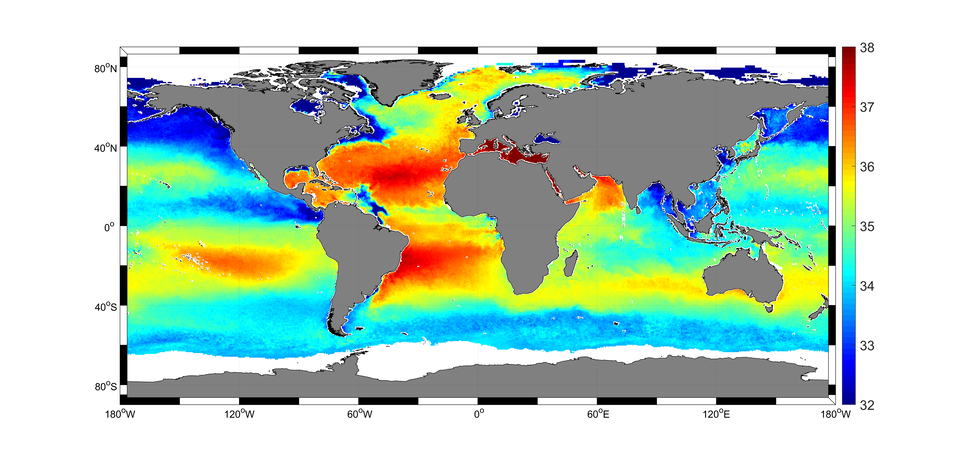
\includegraphics[width=0.75\textwidth]{Figures/salinity_distribution}
    \caption{Global salinity map generated using satellite data~\cite{esa_mapping_salty_waters_2019}.}
    \label{fig:satellite_salinity_map} %chktex 24
\end{figure}
The data measured using this method is reported to be accurate to within $0.1$ on the Practical Salinity Scale PSS-78~\cite{yueh_microwave_salinity_error_sources_2001}, but this method requires multiple different readings to be taken in order to account for the different factors that affect the microwave radiation including \gls{sst}, surface air pressure, surface air temperature, faraday rotation, and surface wind speed~\cite{yueh_microwave_salinity_error_sources_2001}.

\subsection{Salinity from Refractive Index}

The second measurement method that takes advantage of the electromagnetic spectrum interaction with salt water uses the visible light spectrum to measure the refractive index of the water.
The relationship between salinity and refractive index is complex requiring a 27 term equation which includes the effect of pressure and temperature on the water's refractive index.
The refractive index equation is defined a range of $500-700nm$ in wave length, $0-30\degree C$ in temperature, and $0-40$ on the Practical Salinity Scale PSS-78, and $0-11000 dbar$ in pressure.
The equation holds an accuracy of $0.4-80$ \gls{ppm} on the Practical Salinity Scale PSS-78, decreasing with increasing pressure.~\cite{millard_index_of_refraction_algorithm_1990}

A refractometer is the device that is used to measure the refractive index of the water, and due to only needing a small amount of the sample, these devices can be quite compact.
A few researches have developed compact refractometers, the notable ones of which have dimensions of $22.5mm \times 22.5mm \times 120mm$~\cite{malarde_compact_refractometer_2008} and $40mm \times 40mm \times 70mm$~\cite{tengesdal_compact_refractometer_2012} which achieved accuracies of 2 and 83 \gls{ppt} on the Practical Salinity Scale PSS-78 respectively.

\subsection{Salinity from Interferometry}

The last measurement methods that takes advantage or the electromagnetic spectrum interaction with salt water is interferometry.
Interferometry involves generating two identical light waves one the visible spectrum and then passing one through the sample and then comparing the two waves to identify the phase shift and gain.
These measurements can be used to identify the salinity of a sample of salt water~\cite{liao_interferometer_seawater_salinity_2023}.

This method has varying implementation with varying results with \refref{yang_in_situ_refractometer_salinity_measurement_2024} reporting accuracies down to $0.001$ on the Practical Salinity Scale PSS-78 using a Michelson interferometer which other researches have reported other accuracies using different methods~\cite{possetti_interferometer_salinity_measurement_2009}\cite{nguyen_interferometer_salinity_measurement_2009}\cite{zhao_interferometer_salinity_measurement_2009}.
The refractometer does have the disadvantage of being large instrument as the mirrors required to direct the light waves require space and precise alignment making this a difficult method to implement in a compact device. 

\subsection{Salinity from Electromagnetic Induction}

Similarly to conductivity, the magnetic permeability of a liquid is related to the number of ions present in the liquid.
The more ions present in the liquid, the stronger the magnetic field that can be generated by the liquid which increases the magnetic permeability of the liquid which is related to the total dissolved solids in salt water's case~\cite{somaraju_electromagnetic_salinity_2006}.

There are several methods of measuring the magnetic permeability of a liquid that all involve inducing a magnetic field in the liquid and then measuring its response.
These methods all have the advantage of not requiring direct contact with the salt water to make the measurement which allows for the sample to remain undisturbed unlike the conductivity method~\cite{tengesdal_electromagnetic_salinity_2014}.
This method has not been fully investigated however the equipment that is required to measure the magnetic permeability of a liquid is relatively large and requires a lot of power to operate which makes it difficult to implement in a compact device for use in remote environments.

\section{Salinity Measurement Devices using Conductivity}\label{sec:salinity-measurement-devices}
% CTDs, refractometers, conductivity meters, salinometers.

% ----------------------------------------------------
%current CTDs
%
%electrical conductivity sensor https://link.springer.com/article/10.1007/s11270-020-04971-7
%
%arduino version https://www.instructables.com/Water-Salinity-meter/
%
%mini version https://www.diva-portal.org/smash/get/diva2:512332/FULLTEXT01.pdf
%
%% ----------------------------------------------------
%measurement techniques
%
%high res https://link.springer.com/chapter/10.1007/978-1-4615-9182-5_18
%
%salinity and its measurands https://iopscience.iop.org/article/10.1088/1681-7575/aaea92/pdf
%
%interferometer https://iopscience.iop.org/article/10.1088/0957-0233/20/3/034003/meta?casa_token=ZTZbYNUpO0kAAAAA:7jvq44f2kE5qGGEQWt5ji18A7xWG4p9ZT4Ny99eOjMPOfywPIgqRNoCeH0VZby1VjlART_v77WV3rxfwi0k1nwphxfguYA
%
%the whole suite, important for later https://www.researchgate.net/profile/Bjoern-Kjerfve/publication/255660361_Measurement_and_Analysis_of_Water_Current_Temperature_Salinity_and_Density/links/0c9605373c5d3088b4000000/Measurement-and-Analysis-of-Water-Current-Temperature-Salinity-and-Density.pdf
%
%microwave frequency https://www.sensorsportal.com/HTML/DIGEST/january_2014/Vol_162/P_1772.pdf
%
%refraction of light https://www.sciencedirect.com/science/article/abs/pii/S0925400503002922?casa_token=UDq5jm83UIsAAAAA:-UuQMhyBg9tuzleSc8tQnL2vuCv_HYHCB5AicHCTlBkBz_5gipNnDoA6DdPgBL9csU_wWS9lG6Bc
%
%conductivity using electromagnetism https://ieeexplore.ieee.org/abstract/document/7769877
%
%salinity equation paper https://agupubs.onlinelibrary.wiley.com/doi/abs/10.1029/jc083ic01p00466?casa_token=Om_oxKhUgLIAAAAA%3As_ZdT6Qn-zv9SSyC8G3io5r_0mxuepRxFE33jcaLtTNY4tyOQOLAObVtsjeQZ0gPpokwsmrEOP0pPHULQg
%
%% ----------------------------------------------------
%salinity properties
%
%temperature vs salinity https://link.springer.com/article/10.1023/B:EMAS.0000031719.83065.68
%
%salinity and other properties https://pubs.acs.org/doi/10.1021/es402188r
%
%salinity and it antecedents https://ieeexplore.ieee.org/stamp/stamp.jsp?tp=&arnumber=1145448
%
%salinity textbook https://pubs.acs.org/doi/pdf/10.1021/ja02205a013?casa_token=QPyPLh22vacAAAAA:O6Hc1M5FQEDZpJb4oUrGYzboIy0wWn__w6MxXGc8Aw7doPE9tz71yRCbmUtRSP5lOMdTr28U8bYI43IsBg
%
%electrical properties of salt ice https://pubs.acs.org/doi/full/10.1021/jp8055366?casa_token=qvssn_P9p_8AAAAA%3A1FY_4CW5oX_4P9gDNZfp0AaeByCkTF_WOcZ_hLbv2Y2FYsIRsO7ZZkqxzTHTo_MK4vWqfaqqQh2LagyDLA
%
%pressure and temperature increase conductivity https://journals.aps.org/pr/abstract/10.1103/PhysRev.70.329
%
%conductivity vs total dissolved solids https://iopscience.iop.org/article/10.1088/1755-1315/118/1/012019/meta
%
%% ----------------------------------------------------
%producers or CTDs
%
%https://www.whoi.edu/what-we-do/explore/instruments/instruments-sensors-samplers/conductivity-temperature-depth-ctd-sensors/
%
%% ----------------------------------------------------

